\documentclass{school-22.211-notes}
\date{April  9, 2012}

\begin{document}
\maketitle

\lecture{Fission Product Poisoning} \label{fission-product-poisoning}
\topic{Fission Product Chain}
\begin{figure}[ht]
  \centering
  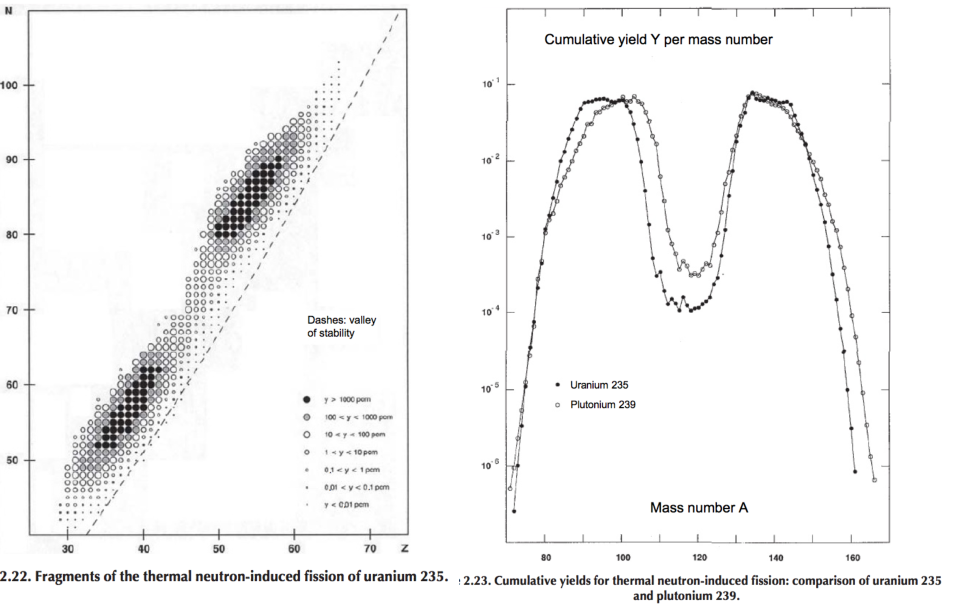
\includegraphics[width=5in]{images/dfs/fission-product-yield.png}
  \caption{Fission Product Yields, Fission Fragments}
\end{figure}

The fission products have the following properties: 
\begin{enumerate}
\item Number: almost all fissions produce precisely two fission produces per fission;
\item Unstability: most fission products are highly unstable and radially decay to other nuclides;
\item Thermal spectrum: some fission produces have large thermal absorption cross sections, which are important for thermal spectrum reactors as in Figure~\ref{major-capture};
\item Fast spectrum: fast reactors are much less sensitive to fission products, because thermal spectrum does not matter. 
\item Distribution: contributing factors are: which species are fissioned (U235, Pu239, etc), the incident fission neutron energy, random statistical fluctuations nuclide breakup.
\item Independent fission yield is a different concept from the cumulative fission yield: the former only accounts for fission yield, whereas the latter accounts for generation of the isotope from independent yield as well as all the precursor isotopes that decay into a specific isotope. 
\item Meda-stable state: an isotope may not directly decay into a stable state; it may branch into a meda-stable state. For our purpose, we are going to take the simplified approach.
\end{enumerate}
\begin{figure}
  \centering
  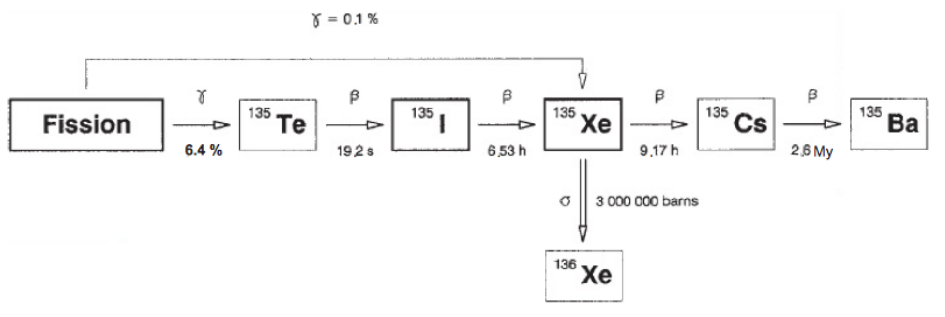
\includegraphics[width=5in]{images/dfs/Xe135.png}
  \caption{I135/Xe135 Chain} \label{Xe135} 
\end{figure}

As an example, we look at the Xenon-135 Chain in Figure~\ref{Xe135}. Typically very rapid transitions are not followed in details when modeling reactor behavior. For instance, because Te's half-life is 19s, we can assume that \ce{^{135}I} is producted instantenously. Most of the chains are similar and are dominated by beta decays until they are stable. 

\begin{figure}
  \centering
  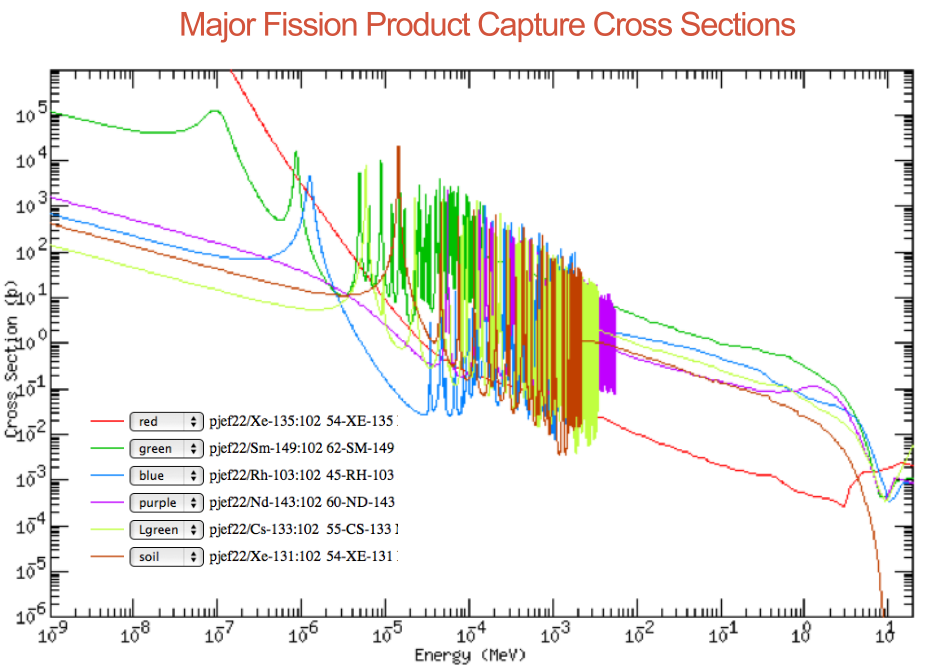
\includegraphics[width=0.59\textwidth]{images/dfs/fission-product-capture-xs.png}
  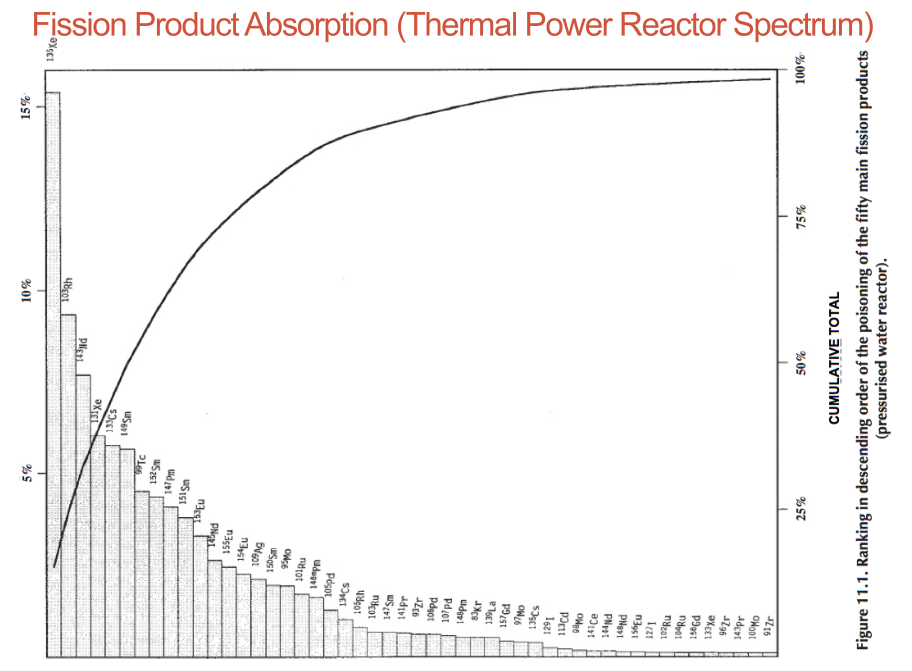
\includegraphics[width=0.59\textwidth]{images/dfs/fission-product-absorption.png}
  \caption{Major Fission Products Absorption} \label{major-capture} 
\end{figure}


\clearpage
\topic{Nuclide Depletion Equation/Neutron Balance Equation}
The numerical solution of nuclide depletion equation is:
\begin{align}
\dNdt + A(t) N(t) &= Y \\
\mbox{IF} &= e^{\int A(t) \dt} = e^{At} \\
e^{At} \dNdt + e^{At} A(t) N(t) &= e^{At} Y \\
\ddt[e^{At} N(t) ] &= e^{At} Y \\
e^{At} N(t) &= A^{-1} e^{At} Y + C 
\end{align}
Using the particular solution that $N_0 = N(t=0)$, then 
\eqn{ N_0 = A^{-1} Y + C \Rightarrow C = N_0 - A^{-1} Y } 
\eqn{ e^{At} N(t) = A^{-1} [e^{At} Y - Y ] + N_0 }
\eqn{ \boxed{ N(t) = e^{-At} N_0 + e^{-At} A^{-1} [e^{At} Y - Y ] } }
We can also write the above differential equation into the matrix form as in Figure~\ref{depletion-matrix}. Notice we asume fission yields, cross sections, and fluxes are constant over the time interval $t_{n-1}, t_n$,
\eqn{ [N(t_n)] = e^{-[A] \Delta t_n} [N(t_{n-1})] + e^{-[A]\Delta t_n} [A]^{-1} [e^{[A] \Delta t_n} Y - Y ] }
\begin{figure}[ht]
  \centering
  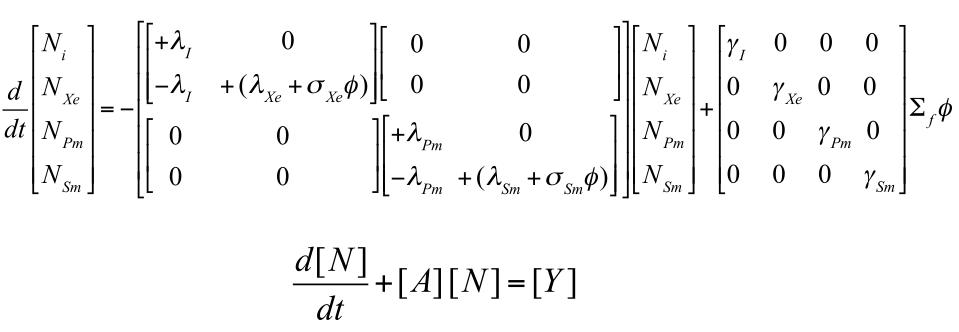
\includegraphics[width=5in]{images/dfs/depletion-matrix-form.png}
  \caption{Nuclide Depletion Equations in Matrix Form} \label{depletion-matrix} 
\end{figure}

\clearpage
\begin{figure}[ht]
  \centering
  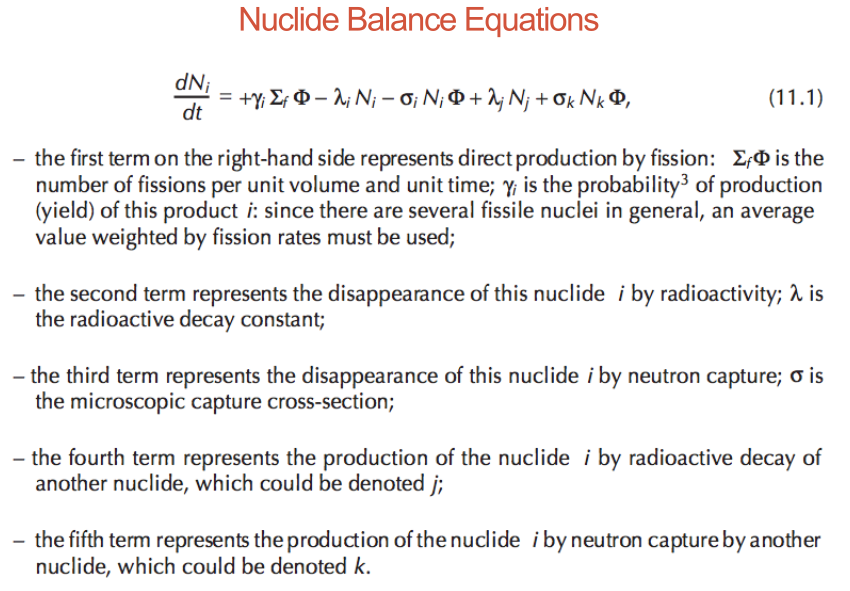
\includegraphics[width=4in]{images/dfs/nuclide-balance-equation.png}
  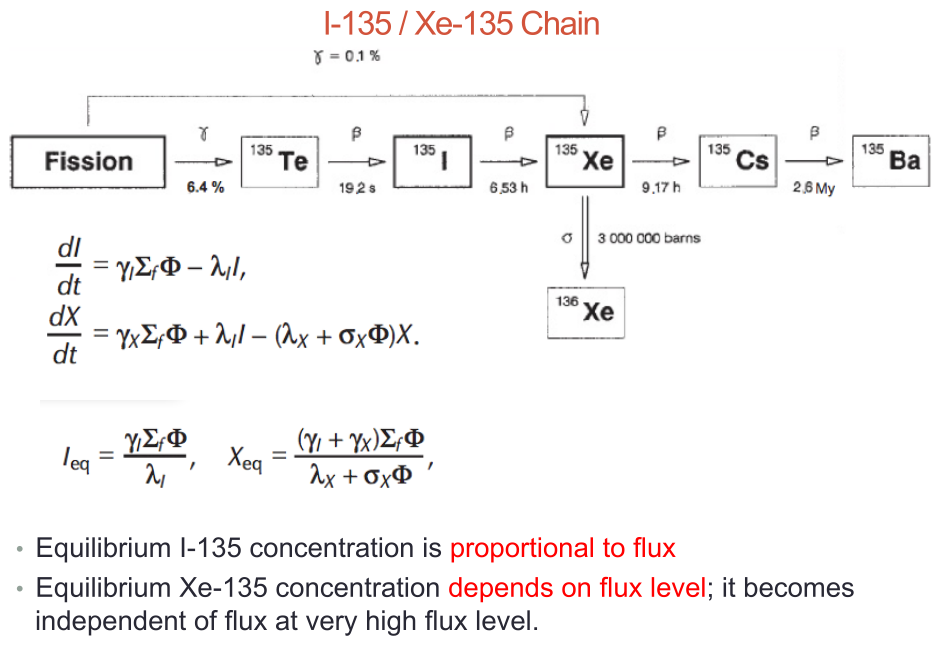
\includegraphics[width=4in]{images/dfs/I-Xe.png}
  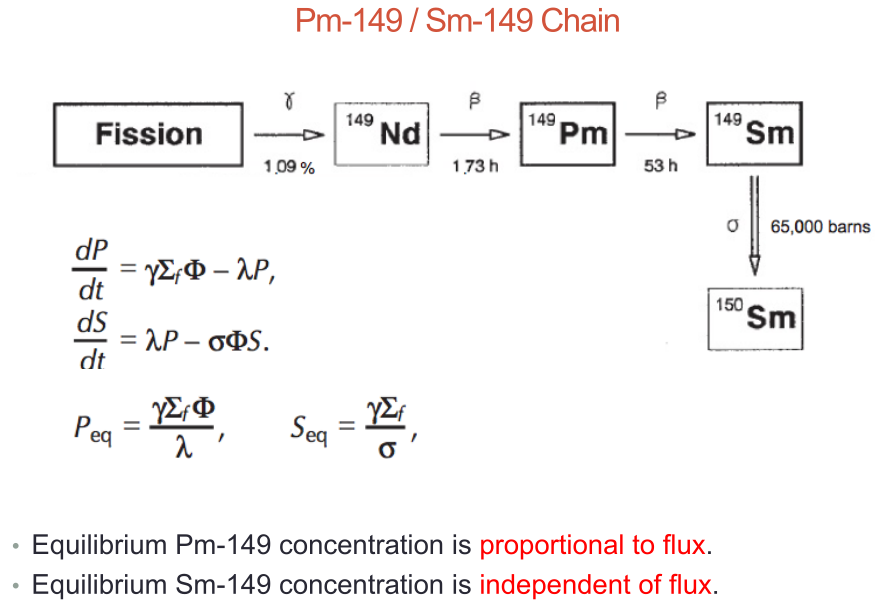
\includegraphics[width=4in]{images/dfs/Pm-Sm.png}
  \caption{Nuclide Balance Equation} \label{nbe} 
\end{figure}



\clearpage
\topic{Iodine/Xenon} \label{FP-Xenon}
Xe-135 has a thermal absorption cross section of $2.6\times 10^6$ barns. 
\begin{itemize}
\item Major source: Iodine decay; \ce{^{135} I ->^{\beta^-} ^{135}Xe} which happens with a half-life of 6.6 hours.
\item Major sink: burnup. Xe has a huge absorption xs ($10^6$ barns), so \ce{^{135} Xe + n -> ^{136} Xe}. Xe can also beta decay again with a half-life of 9.1 hours. 
\end{itemize}
Xenon peaking happens because after shutdown, the major sink is removed, but the major source remains, hence Xenon peaks until the Iodine depletes. Reactors must be designed with enough fuel to offset the effect of Xenon. At the end of core life, there may not be enough reactivity to override peak Xenon; such reactors are called `xenon-precluded.' If a scram occurs, a restart may not be possible for 30-40 hours. See Stacy's Example 6.2 (p.214) for an example of xenon reactivity worth and illustrating diagrams. 



\begin{table}
  \centering
  \begin{tabular}{|p{0.6\textwidth}|p{0.4\textwidth}|}\hline
    \begin{minipage}[b]{0.6\textwidth}
      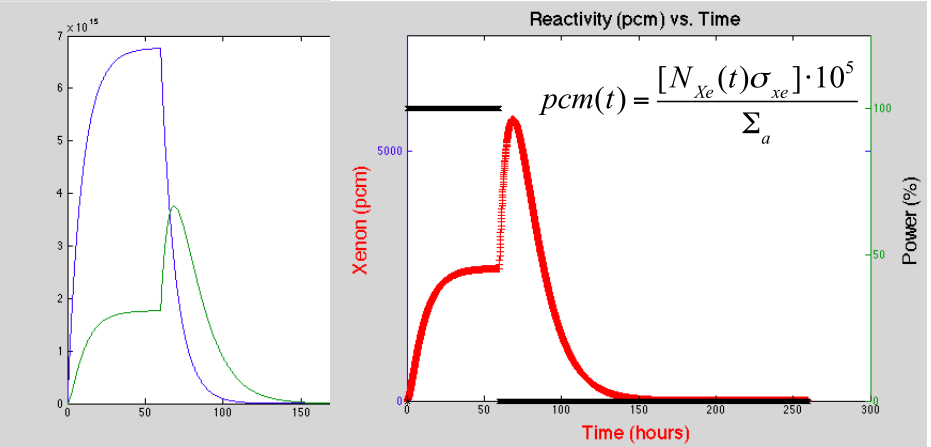
\includegraphics[width=3.5in]{images/dfs/I-Xe-1.png} 
    \end{minipage}
    & 
    \begin{minipage}[b]{0.4\textwidth}
      After startup: both I and Xe increases, and saturates after \hi{30 hrs}. After shutdown: I decays quickly, whereas Xe peaks \hi{9 hrs} after shutdown, and decays away in 60 hours. The peak happens because I coninues to decay into Xe, while Xe can no longer decrease through capture. 
There is a 2.5\% depress due to Xe; the higher the flux, the higher the peak is.
    \end{minipage}   \\ \hline
%
    \begin{minipage}[b]{0.6\textwidth}
      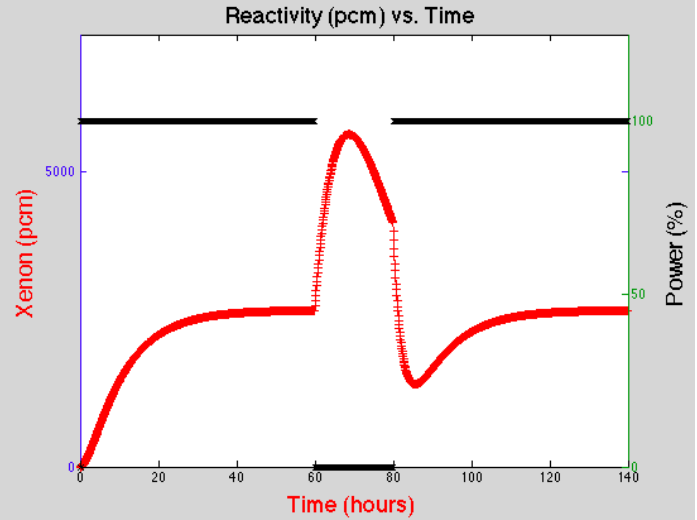
\includegraphics[width=3.5in]{images/dfs/I-Xe-2.png} 
    \end{minipage}
    & 
    \begin{minipage}[b]{0.4\textwidth}    
      A rapid startup after a scram: the concentration decreases immediately after the startup, because Xe absorption increases suddenely due to flux, which over-weights the amount from I decay. Xe would reach its equilibrium value again after about 40 hrs. 
    \end{minipage}  \\ \hline
%
    \begin{minipage}[b]{0.6\textwidth}
      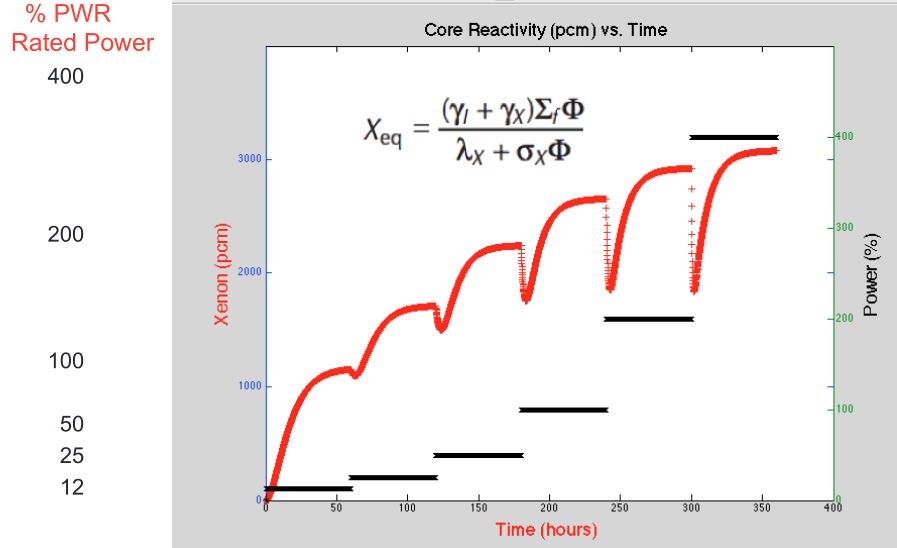
\includegraphics[width=3.5in]{images/dfs/I-Xe-3.png}
    \end{minipage}
 &  
    \begin{minipage}[b]{0.4\textwidth}    
      Equilibrium Xe Worth: if $\phi \to \infty$, then $X_{eq}$ is independent of $\phi$ as shown in the $X_{eq}$ expression; additionally, the Xenon concentration drops right after everytime power increases for the same reason as the previous case (flux increases, the destruction rate of Xe increases instantenously, but the Iodine decay rate has not increased yet). 
    \end{minipage} \\ \hline
%
    \begin{minipage}[b]{0.6\textwidth}
    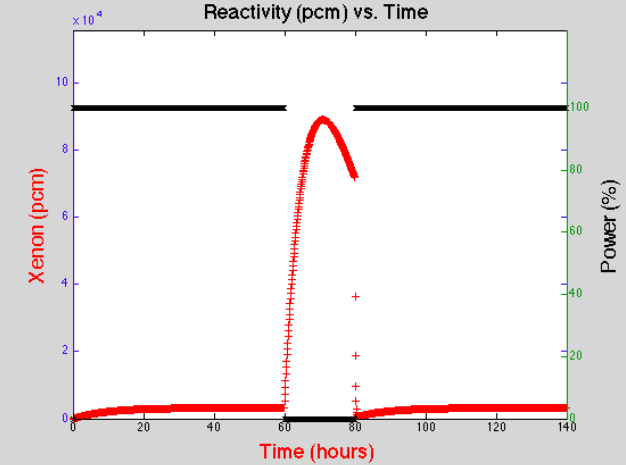
\includegraphics[width=3.5in]{images/dfs/I-Xe-4.png}
    \end{minipage}
 &  
    \begin{minipage}[b]{0.4\textwidth}
      Xe for high flux reactor: Xe peak gives rise to a control constraint. If the reactivity reserves (control rods or poisons that can be removed) are insufficient, the reactor cannot be restarted during this period of increased Xe poisoning. We have to wait till Xe drops to re-start. Alternatively, you can start before Xe builds up, which is pretty rare. 
      \end{minipage} \\ \hline
  \end{tabular}
\end{table}


\clearpage
\topic{Promethium/Samarium} \label{FP-Sm}
Samarium is another fission poisoner. It has one source: decay of Promethium; it has one sink: burnup. 

\begin{table}
  \centering
  \begin{tabular}{|p{0.6\textwidth}|p{0.4\textwidth}|}\hline
    \begin{minipage}[b]{0.6\textwidth}
      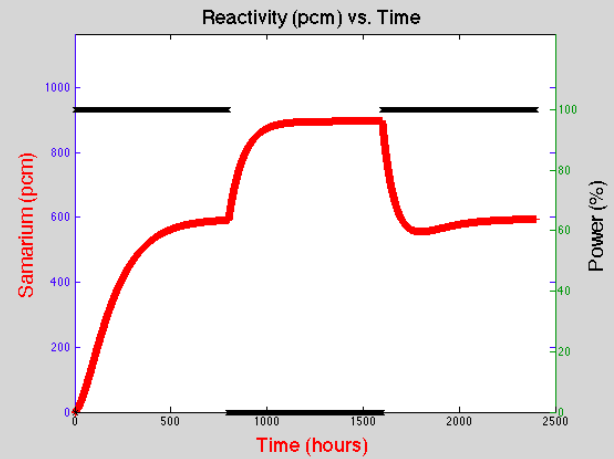
\includegraphics[width=3.5in]{images/dfs/Pm-Sm-1.png} 
    \end{minipage}
    & 
    \begin{minipage}[b]{0.4\textwidth}
      Promethium behaves normally: it builds up and reaches equilibrium when in operation, and it decays away after shutdown. 
Sm behaves similar to Xe in the sense that both peaks after reactor shutdown (Sm peaks \hi{200 hrs} after shutdown, Xe peaks 9 hrs after shutdown). But Sm is stable unlike Xe, and once Pm burns out, Sm would stay constant and never decay away. Sm reactivity peaks by 200-300 pcm after shutdown. 
    \end{minipage}   \\ \hline
%
    \begin{minipage}[b]{0.6\textwidth}
      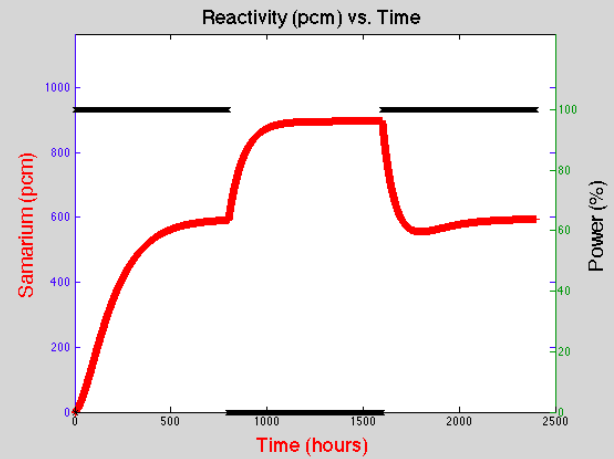
\includegraphics[width=3.5in]{images/dfs/Pm-Sm-2.png} 
    \end{minipage}
    & 
    \begin{minipage}[b]{0.4\textwidth}    
     Sm worth following a refueling outage: Over-write Xenon by pulling the control rods out for a couple of days; then insert the control rods for Sm. Sm returns to equilibrium about 100 hours after restart.
    \end{minipage}  \\ \hline
%
    \begin{minipage}[b]{0.6\textwidth}
      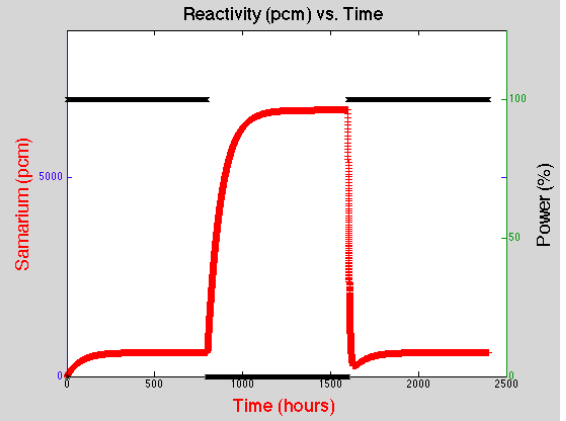
\includegraphics[width=3.5in]{images/dfs/Pm-Sm-3.png}
    \end{minipage}
    &  
    \begin{minipage}[b]{0.4\textwidth}    
      Sm for high flux reactor (20x PWR power density): Sm peaks a lot, which is bad because we may never be able to overrid Sm reactivity without refueling. Hence we should always have a controlled shutdown that burns out Xe/Sm before they build up. 
    \end{minipage} \\ \hline
  \end{tabular}
\end{table}

\clearpage
\topic{Spatial Xenon Oscillations}
When a flux tilt is introduced into a reactor, the Xe concentration will initially increase in the region whose flux is reduced, and initially decrease in the region of increased flux. This shift in the Xe distribution is such as to increase (decrease) the multiplication properties of the region in which the flux has increased (decreased), thus enhancing the flux tilt. After a few hours the increased Xe production due to the increasing I concentration in the high-flux region causes the high-flux region to have reduced multiplicative properties, and vise versa. This decreases, and may reverse, the flux tilt. In this manner it is possible under certain conditions for the delayed Xe production effects to induce growing oscillations in the spatial flux distribution\footnote{Quoted from Stacy's Section 16.6 on page 642}. 

Chasing Xenon, meaning placing the control rods where there are high concentration of Xenon, is wrong because we are nine hours out of sync then. 
\begin{figure}[ht]
  \centering
  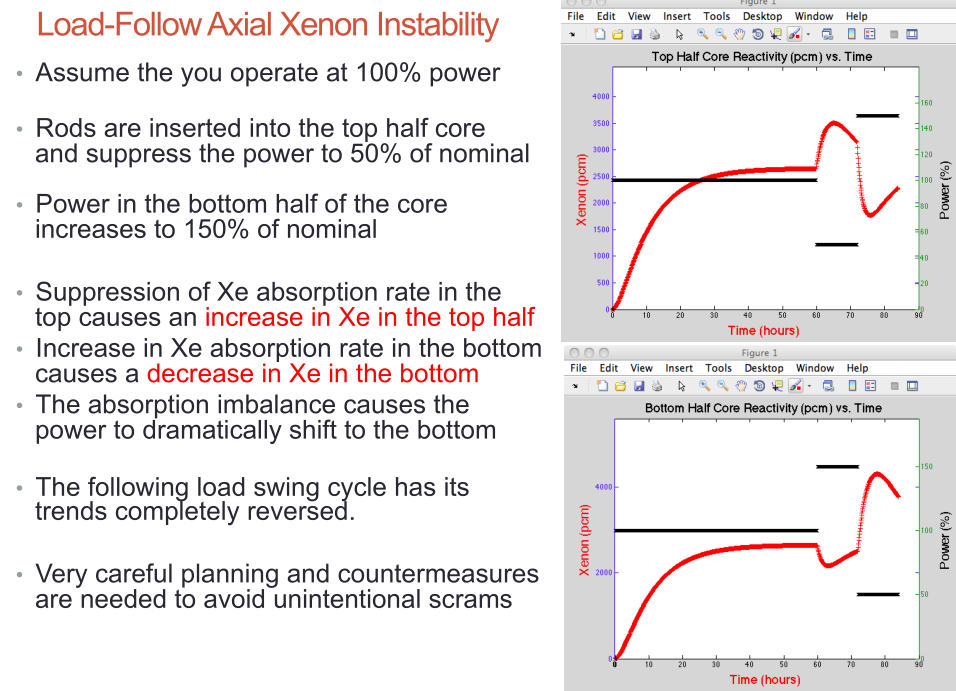
\includegraphics[width=5in]{images/dfs/axial-xenon-instability.png}
\end{figure}

\clearpage
\topic{Production Codes' Fission Product Modeling}
\begin{enumerate}
\item Point Fuel Models: ORIGEN: complete isotropic model. 
\item Lattice Physics: 
  \begin{itemize}
    \item Traditional models: 30 FPs, 2 lumped FPs (these fission products do not saturate; they increase as burnups).
    \item Latest codes: 250 FPs. 
  \end{itemize}
\item Core Models: 
  \begin{itemize}
    \item Traditionally: explicit I/Xe, Pm/Sm, all other FPs are resiual macros (depend on burnups);
    \item Latest codes: about 30 FPs, all other FPs count as residual macros vs. BU. 
  \end{itemize}
\end{enumerate}

Benchmark: Nd is a burnup marker term b/c of its low absorption cross section.   Each fission produces a fixed amount of Nd (Pu and U produces slightly different amount of Nd). Use Nd number density and the yield, you can back out the burnups. 

Gd156 and Gd157 are important for startups when using old rods (15 years old). Once operating, we don't really care about Gd that much. 


\end{document}
